%!TEX program = lualatex
%!TEX encoding = UTF-8 Unicode
\PassOptionsToPackage{french}{babel}
\PassOptionsToPackage{french}{translator}
\documentclass[a4paper,11pt,twoside,french,report]{../common/simplem}
%!TEX root = ./main.tex
%!TEX encoding = UTF-8 Unicode

% Pro­gram­ming fa­cil­i­ties
\usepackage{etoolbox}
\usepackage{ifxetex}
\usepackage{ifluatex}

% Encoding
\usepackage[T1]{fontenc}
\ifboolexpr{bool{xetex} or bool{luatex}}{%
	\usepackage{fontspec}
}{%
	\usepackage[utf8]{inputenc}
}

% Language
\usepackage[french]{babel}
\usepackage[french]{translator}

% General purpose
\usepackage{xcolor}
\usepackage{tcolorbox}
\usepackage{pdflscape}

% Mathematics
\usepackage{amsmath}
\usepackage{amssymb}
\usepackage{mathrsfs}
\usepackage{amsthm}
\usepackage{dsfont}
\usepackage{braket}
\usepackage{stmaryrd}

% Tables
\usepackage{array}
\usepackage{tabularx}
\usepackage{longtable}
\usepackage{tabu}
\usepackage{booktabs}
\usepackage{multirow}
\usepackage{makecell}
\usepackage{blkarray}

% Figures
\usepackage[mode=tex]{standalone}
\usepackage{import}
\usepackage{float}
\usepackage[justification=centering]{caption}

% PGF-TikZ
\usepackage{pgf}
\usepackage{pgfplots}
\pgfplotsset{compat=1.16}
\usepackage{tikz}
\usepackage{tikzpeople}
\usepackage{pgf-umlsd}
\usepackage{pgfgantt}

%!TEX encoding = UTF-8 Unicode

\makeatletter

%----------------------------------------
% Required packages
%----------------------------------------

\usepackage{fontspec} % For Tahoma font
\usepackage{xcolor}
\usepackage{tikz}

%----------------------------------------
% Colors definitions
%----------------------------------------

\definecolor{utbm_cover_background}{RGB}{255,255,255}

\definecolor{utbm_cover_univname}{RGB}{0,0,0}
\definecolor{utbm_cover_univname_text}{RGB}{255,255,255}

\definecolor{utbm_cover_title}{RGB}{125,92,139}
\definecolor{utbm_cover_title_text}{RGB}{255,255,255}

\definecolor{utbm_cover_subtitle}{RGB}{79,78,85}
\definecolor{utbm_cover_subtitle_text}{RGB}{255,255,255}

\definecolor{utbm_cover_main}{RGB}{217,217,87}
\definecolor{utbm_cover_main_text}{RGB}{0,0,0}
\definecolor{utbm_cover_main_shadow_text}{RGB}{153,153,153}

%----------------------------------------
% Font definition
%----------------------------------------

\newfontfamily\tahomafont{Tahoma}

%----------------------------------------
% Default values
%----------------------------------------

%-----
% Default texts and images not related to the student or the company
\newcommand{\@defaultutbmschoolname}{{\bfseries UNIVERSITÉ DE TECHNOLOGIE} DE BELFORT-MONTBÉLIARD}
\newcommand{\@defaultuqacschoolname}{{\bfseries UNIVERSITÉ DU QUÉBEC} À CHICOUTIMI}
\newcommand{\@defaultutbmcompanytutortext}{\iflanguage{french}{Tuteur en entreprise}{Company tutor}}
\newcommand{\@defaultutbmschooltutortext}{\iflanguage{french}{Suiveur UTBM}{UTBM tutor}}
\newcommand{\@defaultuqacschooltutortext}{\iflanguage{french}{Suiveur UQAC}{UQAC tutor}}
\newcommand{\@defaultutbmkeywordstext}{\iflanguage{french}{Mots clefs}{Keywords}}
\newcommand{\@defaultutbmabstracttext}{\iflanguage{french}{Résumé}{Abstract}}
\newcommand{\@defaultutbmschoollogo}{utbm_logo}
\newcommand{\@defaultuqacschoollogo}{uqac_logo}

%-----
% Default texts and images related to the student or the company
\newcommand{\@defaultutbmfrontillustration}{utbm_default_illustration}
\newcommand{\@defaultutbmfrontillustrationwidth}{width=\paperwidth}
\newcommand{\@defaultutbmfrontillustrationyshift}{0pt}
\newcommand{\@defaultutbmtitle}{\iflanguage{french}{Titre}{Title}}
\newcommand{\@defaultutbmsubtitle}{\iflanguage{french}{Sous-titre}{Subtitle}}
\newcommand{\@defaultutbmstudent}{\iflanguage{french}{Nom Étudiant}{Student name}}
\newcommand{\@defaultutbmstudentdepartment}{\iflanguage{french}{Département UTBM}{UTBM department}}
\newcommand{\@defaultuqacstudentdepartment}{\iflanguage{french}{Département UQAC}{UQAC department}}
\newcommand{\@defaultutbmstudentpathway}{\iflanguage{french}{Filière UTBM}{UTBM pathway}}
\newcommand{\@defaultuqacstudentpathway}{\iflanguage{french}{Filière UQAC}{UQAC pathway}}
\newcommand{\@defaultutbmcompany}{\iflanguage{french}{Entreprise}{Company}}
\newcommand{\@defaultutbmcompanyaddress}{\iflanguage{french}{Adresse}{Address}}
\newcommand{\@defaultutbmcompanywebsite}{\iflanguage{french}{Site web}{Website}}
\newcommand{\@defaultutbmcompanytutor}{\iflanguage{french}{Nom tuteur en entreprise}{Company tutor name}}
\newcommand{\@defaultutbmschooltutor}{\iflanguage{french}{Nom suiveur UTBM}{UTBM tutor name}}
\newcommand{\@defaultuqacschooltutor}{\iflanguage{french}{Nom suiveur UQAC}{UQAC tutor name}}
\newcommand{\@defaultutbmkeywords}{\iflanguage{french}{Liste de mots clefs}{List of keywords}}
\newcommand{\@defaultutbmabstract}{\iflanguage{french}{Texte du résumé}{Abstract text}}

%----------------------------------------
% Configuration commands
%----------------------------------------
% Commands to set the texts and images not related to the student or the company
% Default configuration for English and French languages, use the commands for other languages

%-----
% Set the UTBM school name
% \setutbmschoolname{name}
\newcommand{\setutbmschoolname}[1]{\renewcommand{\@utbmschoolname}{#1}}
\newcommand{\@utbmschoolname}{\@defaultutbmschoolname}

%-----
% Set the UQAC school name
% \setuqacschoolname{name}
\newcommand{\setuqacschoolname}[1]{\renewcommand{\@uqacschoolname}{#1}}
\newcommand{\@uqacschoolname}{\@defaultuqacschoolname}

%-----
% Set the text for the company tutor
% \setutbmcompanytutortext{text}
\newcommand{\setutbmcompanytutortext}[1]{\renewcommand{\@utbmcompanytutortext}{#1}}
\newcommand{\@utbmcompanytutortext}{\@defaultutbmcompanytutortext}

%-----
% Set the text for the UTBM school tutor
% \setutbmschooltutortext{text}
\newcommand{\setutbmschooltutortext}[1]{\renewcommand{\@utbmschooltutortext}{#1}}
\newcommand{\@utbmschooltutortext}{\@defaultutbmschooltutortext}

%-----
% Set the text for the UQAC school tutor
% \setuqacschooltutortext{text}
\newcommand{\setuqacschooltutortext}[1]{\renewcommand{\@uqacschooltutortext}{#1}}
\newcommand{\@uqacschooltutortext}{\@defaultuqacschooltutortext}

%-----
% Set the text for the keywords
% \setutbmkeywordstext{text}
\newcommand{\setutbmkeywordstext}[1]{\renewcommand{\@utbmkeywordstext}{#1}}
\newcommand{\@utbmkeywordstext}{\@defaultutbmkeywordstext}

%-----
% Set the text for the abstract
% \setutbmabstracttext{text}
\newcommand{\setutbmabstracttext}[1]{\renewcommand{\@utbmabstracttext}{#1}}
\newcommand{\@utbmabstracttext}{\@defaultutbmabstracttext}

%-----
% Set the UTBM school logo (the file name can be as in the \includegraphics command)
% \setutbmschoollogo{filename}
\newcommand{\setutbmschoollogo}[1]{\renewcommand{\@utbmschoollogo}{#1}}
\newcommand{\@utbmschoollogo}{\@defaultutbmschoollogo}

%-----
% Set the UQAC school logo (the file name can be as in the \includegraphics command)
% \setuqacschoollogo{filename}
\newcommand{\setuqacschoollogo}[1]{\renewcommand{\@uqacschoollogo}{#1}}
\newcommand{\@uqacschoollogo}{\@defaultuqacschoollogo}

%----------------------------------------
% Informations setting commands
%----------------------------------------
% Commands to set the texts and images related to the student or the company
% Default configuration can be used to see where will be displayed each information
% but the commands should be used to set the cover informations

%-----
% Set the illustration figure on the front page (the file name can be as in the \includegraphics command)
% \setutbmfrontillustration{filename}
\newcommand{\setutbmfrontillustration}[1]{\renewcommand{\@utbmfrontillustration}{#1}}
\newcommand{\@utbmfrontillustration}{\@defaultutbmfrontillustration}

%-----
% Set the illustration figure options (options for the \includegraphics command)
% \setutbmfrontillustrationwidth{options}
\newcommand{\setutbmfrontillustrationwidth}[1]{\renewcommand{\@utbmfrontillustrationwidth}{#1}}
\newcommand{\@utbmfrontillustrationwidth}{\@defaultutbmfrontillustrationwidth}

%-----
% Set the illustration figure y shift from the top of the page
% \setutbmfrontillustrationyshift{yshift}
\newcommand{\setutbmfrontillustrationyshift}[1]{\renewcommand{\@utbmfrontillustrationyshift}{#1}}
\newcommand{\@utbmfrontillustrationyshift}{\@defaultutbmfrontillustrationyshift}

%-----
% Set the title
% \setutbmtitle{title}
\newcommand{\setutbmtitle}[1]{\renewcommand{\@utbmtitle}{#1}}
\newcommand{\@utbmtitle}{\@defaultutbmtitle}

%-----
% Set the subtitle
% \setutbmsubtitle{subtitle}
\newcommand{\setutbmsubtitle}[1]{\renewcommand{\@utbmsubtitle}{#1}}
\newcommand{\@utbmsubtitle}{\@defaultutbmsubtitle}

%-----
% Set the student
% \setutbmstudent{name}
\newcommand{\setutbmstudent}[1]{\renewcommand{\@utbmstudent}{#1}}
\newcommand{\@utbmstudent}{\@defaultutbmstudent}

%-----
% Set the student UTBM department
% \setutbmstudentdepartment{department}
\newcommand{\setutbmstudentdepartment}[1]{\renewcommand{\@utbmstudentdepartment}{#1}}
\newcommand{\@utbmstudentdepartment}{\@defaultutbmstudentdepartment}

%-----
% Set the student UQAC department
% \setuqacstudentdepartment{department}
\newcommand{\setuqacstudentdepartment}[1]{\renewcommand{\@uqacstudentdepartment}{#1}}
\newcommand{\@uqacstudentdepartment}{\@defaultuqacstudentdepartment}

%-----
% Set the student UTBM pathway
% \setutbmstudentpathway{pathway}
\newcommand{\setutbmstudentpathway}[1]{\renewcommand{\@utbmstudentpathway}{#1}}
\newcommand{\@utbmstudentpathway}{\@defaultutbmstudentpathway}

%-----
% Set the student UQAC pathway
% \setuqacstudentpathway{pathway}
\newcommand{\setuqacstudentpathway}[1]{\renewcommand{\@uqacstudentpathway}{#1}}
\newcommand{\@uqacstudentpathway}{\@defaultuqacstudentpathway}

%-----
% Set the company
% \setutbmcompany{name}
\newcommand{\setutbmcompany}[1]{\renewcommand{\@utbmcompany}{#1}}
\newcommand{\@utbmcompany}{\@defaultutbmcompany}

%-----
% Set the company address
% \setutbmcompanyaddress{address}
\newcommand{\setutbmcompanyaddress}[1]{\renewcommand{\@utbmcompanyaddress}{#1}}
\newcommand{\@utbmcompanyaddress}{\@defaultutbmcompanyaddress}

%-----
% Set the company website
% \setutbmcompanywebsite{website}
\newcommand{\setutbmcompanywebsite}[1]{\renewcommand{\@utbmcompanywebsite}{#1}}
\newcommand{\@utbmcompanywebsite}{\@defaultutbmcompanywebsite}

%-----
% Set the company tutor
% \setutbmcompanytutor{tutor}
\newcommand{\setutbmcompanytutor}[1]{\renewcommand{\@utbmcompanytutor}{#1}}
\newcommand{\@utbmcompanytutor}{\@defaultutbmcompanytutor}

%-----
% Set the UTBM school tutor
% \setutbmschooltutor{tutor}
\newcommand{\setutbmschooltutor}[1]{\renewcommand{\@utbmschooltutor}{#1}}
\newcommand{\@utbmschooltutor}{\@defaultutbmschooltutor}

%-----
% Set the UQAC school tutor
% \setuqacschooltutor{tutor}
\newcommand{\setuqacschooltutor}[1]{\renewcommand{\@uqacschooltutor}{#1}}
\newcommand{\@uqacschooltutor}{\@defaultuqacschooltutor}

%-----
% Set the keywords
% \setutbmkeywords{keywords}
\newcommand{\setutbmkeywords}[1]{\renewcommand{\@utbmkeywords}{#1}}
\newcommand{\@utbmkeywords}{\@defaultutbmkeywords}

%-----
% Set the abstract
% \setutbmabstract{abstract}
\newcommand{\setutbmabstract}[1]{\renewcommand{\@utbmabstract}{#1}}
\newcommand{\@utbmabstract}{\@defaultutbmabstract}

%----------------------------------------
% Cover generation commands
%----------------------------------------

%-----
% Make the front cover
% \makeutbmfrontcover[shift]
\newcommand{\makeutbmfrontcover}[1][(0,0)]{
	\clearpage
	\thispagestyle{empty}
	\parindent0pt
	\begin{tikzpicture}[remember picture,overlay]
		\tikzset{
			utbm text/.style={
				text badly ragged,
				inner xsep=1cm,
				outer sep=0pt,
				text width=\paperwidth-2cm,
				anchor=north,
			},
			utbm rectangle/.style={
				rectangle,
				inner sep=0pt,
				outer sep=0pt,
				anchor=north,
				minimum width=\paperwidth,
			}
		}

		\node[
			shift={#1},
			inner sep=0pt,
			anchor=north,
			minimum width=\paperwidth,
			minimum height=\paperheight,
		]
		(anchor) at (current page.north)
		{};

		\node[
			utbm rectangle,
			fill=utbm_cover_background,
			minimum height=\paperheight,
		]
		(background) at (anchor.north)
		{};

		% Hide illustration if too hight
		\node[
			yshift=-8.6cm,
			utbm rectangle,
			fill=utbm_cover_background,
			minimum height=\paperheight-8.6cm,
		]
		(background2) at (anchor.north)
		{};

		\node[
			yshift=\@utbmfrontillustrationyshift,
			inner sep=0pt,
			anchor=north,
		]
		(illustration) at (anchor.north)
		{\includegraphics[width=\@utbmfrontillustrationwidth]{\@utbmfrontillustration}};

		\node[
			yshift=-7.6cm,
			utbm text,
			fill=utbm_cover_univname,
			text=utbm_cover_univname_text,
			minimum height=0.8cm,
		]
		(schoolname) at (anchor.north)
		{\tahomafont\fontsize{14.4}{17.2}\selectfont {\@utbmschoolname}\\{\@uqacschoolname}};

		\node[utbm text,
			fill=utbm_cover_title,
			text=utbm_cover_title_text,
			minimum height=2.8cm,
		]
		(title) at (schoolname.south)
		{\tahomafont\fontsize{24}{29}\selectfont \bfseries \@utbmtitle};

		\node[utbm text,
			fill=utbm_cover_subtitle,
			text=utbm_cover_subtitle_text,
			minimum height=0.8cm,
		]
		(subtitle) at (title.south)
		{\tahomafont\fontsize{12}{14}\selectfont \bfseries \@utbmsubtitle};

		\node[
			utbm rectangle,
			fill=utbm_cover_main,
			minimum height=13.65cm,
		]
		(information) at (subtitle.south)
		{};

		\node[
			yshift=-1.3cm,
			utbm text,
			text=black,
			minimum height=0.8cm,
		]
		(student) at (subtitle.south)
		{\tahomafont\bfseries {\fontsize{18}{22}\selectfont \@utbmstudent}};

		\node[
			yshift=-2.4cm,
			utbm text,
			text=black,
			minimum height=0.8cm,
		]
		(studentutbminfo) at (subtitle.south)
		{\tahomafont\bfseries\fontsize{10}{12}\selectfont{\fontsize{12}{14}\selectfont UTBM}\\
		\@utbmstudentdepartment\\
		{\color{utbm_cover_main_shadow_text}\@utbmstudentpathway}};

		\node[
			yshift=-2.4cm,
			xshift=10cm,
			utbm text,
			text=black,
			minimum height=0.8cm,
		]
		(studentuqacinfo) at (subtitle.south)
		{\tahomafont\bfseries\fontsize{10}{12}\selectfont{\fontsize{12}{14}\selectfont UQAC}\\
		\@uqacstudentdepartment\\
		{\color{utbm_cover_main_shadow_text}\@uqacstudentpathway}};

		\node[
			yshift=-6cm,
			utbm text,
			text=utbm_cover_main_text,
			minimum height=0.8cm,
		]
		(company) at (subtitle.south)
		{\tahomafont\bfseries {\fontsize{20}{24}\selectfont \@utbmcompany}\\\vspace{0.3cm}
		{\fontsize{12}{14}\selectfont\color{utbm_cover_main_shadow_text} \@utbmcompanyaddress\\\vspace{0.1cm}
		\@utbmcompanywebsite}};

		\node[
			yshift=-10.8cm,
			utbm text,
			text=utbm_cover_main_text,
			minimum height=0.8cm,
		]
		(company_tutor) at (subtitle.south)
		{\tahomafont {\fontsize{12}{14}\selectfont\color{utbm_cover_main_shadow_text} \@utbmcompanytutortext}\\
		\vspace*{0.7mm}{\fontsize{14}{17}\selectfont\bfseries \@utbmcompanytutor}};

		\node[
			yshift=-10.8cm,
			utbm text,
			align=right,
			text=utbm_cover_main_text,
			minimum height=0.8cm,
		]
		(school_tutor) at (subtitle.south)
		{\tahomafont {\fontsize{12}{14}\selectfont\color{utbm_cover_main_shadow_text} \@uqacschooltutortext}\\
		\vspace*{0.7mm}{\fontsize{14}{17}\selectfont\bfseries \@uqacschooltutor}};

		\node[
			yshift=-8.8cm,
			utbm text,
			align=right,
			text=utbm_cover_main_text,
			minimum height=0.8cm,
		]
		(school_tutor) at (subtitle.south)
		{\tahomafont {\fontsize{12}{14}\selectfont\color{utbm_cover_main_shadow_text} \@utbmschooltutortext}\\
		\vspace*{0.7mm}{\fontsize{14}{17}\selectfont\bfseries \@utbmschooltutor}};

		\node[
			yshift=0.7cm,
			xshift=-1cm,
			inner sep=0pt,
			anchor=south east,
		]
		(schoollogo) at (anchor.south east)
		{\includegraphics[width=5.18cm]{\@utbmschoollogo}};

		\node[
			yshift=0.4cm,
			xshift=1cm,
			inner sep=0pt,
			anchor=south west,
		]
		(schoollogo) at (anchor.south west)
		{\includegraphics[width=4.5cm]{\@uqacschoollogo}};


		% \node[
		% 	rectangle,
		% 	red,
		% 	fill=red,
		% 	inner sep=0pt,
		% 	anchor=north,
		% 	minimum width=\paperwidth,
		% 	minimum height=\paperheight,
		% ]
		% (anchor) at (current page.north)
		% {};
	\end{tikzpicture}
	\newpage{}
}

%-----
% Make the back cover
% \makeutbmbackcover[shift]
\newcommand{\makeutbmbackcover}[1][(0,0)]{
	\clearpage \ifodd\value{page}\hbox{}\newpage\fi
	\thispagestyle{empty}
	\parindent0pt
	\begin{tikzpicture}[remember picture,overlay]
		\tikzset{
			utbm text/.style={
				text badly ragged,
				inner xsep=1cm,
				outer sep=0pt,
				text width=\paperwidth-2cm,
			},
			utbm rectangle/.style={
				rectangle,
				inner sep=0pt,
				outer sep=0pt,
				anchor=north,
				minimum width=\paperwidth,
			}
		}

		\node[
			shift={#1},
			inner sep=0pt,
			anchor=north,
			minimum width=\paperwidth,
			minimum height=\paperheight,
		]
		(anchor) at (current page.north)
		{};

		\node[
			utbm rectangle,
			fill=utbm_cover_background,
			minimum height=\paperheight,
		]
		(background) at (anchor.north)
		{};

		\node[
			yshift=-8.4cm,
			utbm rectangle,
			fill=utbm_cover_subtitle,
			minimum height=1cm,
		]
		(line) at (anchor.north)
		{};

		\node[
			utbm rectangle,
			fill=utbm_cover_main,
			minimum height=17.25cm,
		]
		(information) at (line.south)
		{};

		\node[
			yshift=-1.5cm,
			utbm text,
			text=utbm_cover_main_text,
			anchor=north,
			minimum height=0.8cm,
		]
		(keywords) at (anchor.north)
		{\tahomafont\fontsize{12}{14}\selectfont {\bfseries \@utbmkeywordstext}\\
		\hfil\\
		\@utbmkeywords};

		\node[
			yshift=0.25cm,
			utbm text,
			text=utbm_cover_main_text,
			anchor=south,
			minimum height=0.8cm,
		]
		(student) at (line.north)
		{\tahomafont\fontsize{14}{17}\selectfont\bfseries \@utbmstudent};

		\node[
			yshift=0.25cm,
			utbm text,
			align=right,
			text=utbm_cover_main_text,
			anchor=south,
			minimum height=0.8cm,
		]
		(subtitle) at (line.north)
		{\tahomafont\fontsize{14}{17}\selectfont\bfseries \@utbmsubtitle};

		\node[
			yshift=-1.2cm,
			utbm text,
			text justified,
			text=utbm_cover_main_text,
			anchor=north,
			minimum height=0.8cm,
		]
		(abstract) at (information.north)
		{\tahomafont\fontsize{12}{14}\selectfont {\bfseries \@utbmabstracttext}\\
		\hfil\\
		\@utbmabstract};

		\node[
			yshift=0.5cm,
			utbm text,
			text=utbm_cover_main_text,
			anchor=south,
			minimum height=0.8cm,
		]
		(company) at (information.south)
		{\tahomafont\bfseries {\fontsize{20}{24}\selectfont \@utbmcompany}\\\vspace{0.3cm}
		{\fontsize{12}{14}\selectfont\color{utbm_cover_main_shadow_text} \@utbmcompanyaddress\\\vspace{0.1cm}
		\@utbmcompanywebsite}};

		\node[
			yshift=0.5cm,
			xshift=-1cm,
			inner sep=0pt,
			anchor=south east,
		]
		(schoollogo) at (anchor.south east)
		{\includegraphics[width=5.18cm]{\@utbmschoollogo}};

		\node[
			yshift=0.2cm,
			xshift=1cm,
			inner sep=0pt,
			anchor=south west,
		]
		(schoollogo) at (anchor.south west)
		{\includegraphics[width=4.5cm]{\@uqacschoollogo}};
	\end{tikzpicture}
}

\makeatother

%!TEX encoding = UTF-8 Unicode

% C++
\newcommand{\Cpp}{\texorpdfstring{C\kern-0.05em\protect\raisebox{.35ex}{\textsmaller[2]{+\kern-0.05em+}}}{C++}}

% Clear to the next left page
\newcommand*{\cleartoleftpage}{
  \clearpage \ifodd\value{page}\hbox{}\newpage\fi
}

%!TEX root = ./main.tex
%!TEX encoding = UTF-8 Unicode

%----------------------------------------
% Informations
%----------------------------------------

\title{Métaheuristiques Hybrides pour le problème de couverture par ensembles}
\author{Maxime Pinard}
\date{2020}

%----------------------------------------
% Covers configuration
%----------------------------------------

\setutbmfrontillustration{IRIMAS}
\setutbmfrontillustrationwidth{0.9\paperwidth}
\setutbmfrontillustrationyshift{-2cm}

\setutbmtitle{Métaheuristiques Hybrides pour le problème de couverture par ensembles}
\setutbmsubtitle{Rapport de stage ST50 / 8INF859 - P2020}

\setutbmstudent{Maxime Pinard}
\setutbmstudentdepartment{Département Informatique}
\setutbmstudentpathway{Filière Interaction Imagerie Réalité Virtuelle}
\setuqacstudentdepartment{Département d'Informatique et de Mathématique}
\setuqacstudentpathway{Maîtrise en Informatique Profil Professionnel}

\setutbmcompany{Institut de Recherche en Informatique, Mathématiques, Automatique et Signal}
\setutbmcompanyaddress{12 rue des Frères Lumière\\68 093 MULHOUSE Cedex}
\setutbmcompanywebsite{\href{https://www.irimas.uha.fr/}{\color{utbm_cover_main_shadow_text}{https://www.irimas.uha.fr/}}}

\setutbmcompanytutor{Laurent Moalic}
\setutbmschooltutor{Fabrice Lauri}
\setuqacschooltutor{Sara Séguin}

\setutbmkeywords{
	recherche \textendash{}	mathématiques \textendash{} informatique \textendash{} optimisation \textendash{} métaheuristique \textendash{} problème de couverture par ensembles
}
\setutbmabstract{
	Le problème de « couverture par ensembles », également connu sous le nom de « set covering problem », fait partie des grands classiques de l’optimisation. Au sein de l’institut de recherche IRIMAS, nous nous intéressons notamment aux approches heuristiques permettant de résoudre de tels
	problèmes.
	\vspace{12pt}\\
	Dans le cadre de ce stage, nous nous intéressons au développement de méthodes hybrides de type mémétique, mêlant recherche locale et algorithmes génétiques. Ce type d’hybridation s’est révélé particulièrement efficace pour résoudre des problèmes connus pour être très difficiles, appartenant à la famille des problèmes NP-complets. Dans le cadre de travaux menés conjointement avec l’ENAC de Toulouse, nous avons développé des algorithmes reposant sur des populations réduites à deux individus. Les résultats obtenus sur le problème bien connu de coloration de graphes nous laisse supposer que cette démarche pourrait se révéler particulièrement efficace sur d’autres types de problèmes, tels que le « set cover ».
}

%----------------------------------------
% Configuration
%----------------------------------------

% reduce underscores size
\renewcommand{\_}{\textscale{.5}{\textunderscore}}

%----------------------------------------
% Figures
%----------------------------------------

% Common file
%!TEX encoding = UTF-8 Unicode

\usetikzlibrary{shapes}
\usetikzlibrary{arrows.meta}
\usetikzlibrary{calc}

\definecolor{bg_color}{RGB}{250,250,229}

\colorlet{color1}{cyan!50}
\colorlet{color2}{red!30!green!40}
\colorlet{color3}{orange!50}
\colorlet{color4}{violet!60!blue!55}

\definecolor{Cblue}{RGB}{38,75,150}
\definecolor{Cgreen}{RGB}{39,179,118}
\definecolor{Cdarkgreen}{RGB}{0,111,60}
\definecolor{Corange}{RGB}{249,167,62}
\definecolor{Cred}{RGB}{191,33,47}

\newganttlinktype{bartobardown}{
	\ganttsetstartanchor{south east}
	\ganttsetendanchor{north west}
	\draw [/pgfgantt/link] (\xLeft, \yUpper) -- (\xRight, \yLower);
}
\newganttlinktype{bartobarup}{
	\ganttsetstartanchor{north east}
	\ganttsetendanchor{south west}
	\draw [/pgfgantt/link] (\xLeft, \yUpper) -- (\xRight, \yLower);
}
\newganttlinktype{milestonetobardown}{
	\ganttsetstartanchor{south}
	\ganttsetendanchor{north west}
	\draw [/pgfgantt/link] (\xLeft, \yUpper) -- (\xRight, \yLower);
}
\newganttlinktype{bartomilestonedown}{
	\ganttsetstartanchor{south east}
	\ganttsetendanchor{north}
	\draw [/pgfgantt/link] (\xLeft, \yUpper) -- (\xRight, \yLower);
}


% Figures folder
\graphicspath{{../figures/}}

% Figures counting
\counterwithout{figure}{chapter}

%----------------------------------------
% Tables
%----------------------------------------

% Common file
%!TEX encoding = UTF-8 Unicode


% Table counting
\counterwithout{table}{chapter}

%----------------------------------------
% Plots
%----------------------------------------

%\pgfplotsset{
%  table/search path={../plots},
%}

%----------------------------------------
% Boxes
%----------------------------------------

\tcbuselibrary{most}
\newtcolorbox{infobox}[2][]{
	breakable,
	colback=gray!5!,
	colframe=black!75!white,
	arc=0pt,
	title=#2,
	#1
}

%----------------------------------------
% Commands
%----------------------------------------

\newcommand{\solver}{\textit{solver}}
\newcommand{\printer}{\textit{printer}}
\newcommand{\common}{\textit{common}}


%----------------------------------------
% Bibliography
%----------------------------------------
\addbibresource{../references/references.bib}
%\nocite{*}

%----------------------------------------
% Glossary
%----------------------------------------
\makeglossaries
%!TEX encoding = UTF-8 Unicode

\newacronym{8INF808}{8INF808}{Informatique appliquée et optimisation}
\newacronym{8INF852}{8INF852}{Métaheuristiques en optimisation}
\newacronym{8INF859}{8INF859}{Stage}
\newacronym{8INF870}{8INF870}{Algorithmique}
\newacronym{AG41}{AG41}{Optimisation et recherche opérationnelle}
\newacronym{ARCHIMEDE}{ARCHIMEDE}{Archéologie et Histoire de la Méditerranée et de l’Europe}
\newacronym{BETA}{BETA}{Bureau d’Économie Théorique Appliquée}
\newacronym{BKS}{BKS}{Best Known Solution}
\newacronym{CERDACC}{CERDACC}{Centre Européen de Recherche sur les Droits des Accidents Collectifs et Catastrophes}
\newacronym{CFAU}{CFAU}{Centre de Formation d'Apprentis Universitaire}
\newacronym{CLAM}{CLAM}{service de Certifications et Langues par Apprentissage Multimédia}
\newacronym{CREGO}{CREGO}{Centre de Recherche en Gestion des Organisations}
\newacronym{CRESAT}{CRESAT}{Centre de Recherche sur les Économies, les Sociétés, les Arts et les Technologies}
\newacronym{CUFEF}{CUFEF}{Centre Universitaire de Formation des Enseignants et des Formateurs}
\newacronym{DIMACS}{DIMACS}{Center for Discrete Mathematics and Theoretical Computer Science}
\newacronym{DIM}{DIM}{Département d'Informatique et de Mathématique}
\newacronym{DUT}{DUT}{Diplômes Universitaires de Technologie}
\newacronym{EA2019}{EA2019}{14\textsuperscript{th} Biennial International Conference on Artificial Evolution}
\newacronym{ENSCMu}{ENSCMu}{École Nationale Supérieure de Chimie de Mulhouse}
\newacronym{ENSISA}{ENSISA}{École Nationale Supérieure d'Ingénieurs Sud Alsace}
\newacronym{Equip@meso}{Equip@meso}{Equipement d’excellence de calcul intensif de Mésocentres coordonnés}
\newacronym{FIFO}{FIFO}{First In First Out}
\newacronym{FLSH}{FLSH}{Faculté des Lettres, Langues et Sciences Humaines}
\newacronym{FMA}{FMA}{Faculté de Marketing et d'Agrosciences}
\newacronym{FOTI}{FOTI}{Fonctions Optiques et Traitement des Images}
\newacronym{FSESJ}{FSESJ}{Faculté des Sciences Économiques Sociales et Juridiques}
\newacronym{FST}{FST}{Faculté des Sciences et Techniques}
\newacronym{GRE}{GRE}{Laboratoire Gestion des Risques et Environnement}
\newacronym{GVCP}{GVCP}{Graph Vertex Coloring Problem}
\newacronym{HEAD}{HEAD}{Hybrid Evolutionary Algorithm in Duet}
\newacronym{HEA}{HEA}{Hybrid Evolutionary Algorithm}
\newacronym{HPC}{HPC}{High-Performance Computing}
\newacronym{IDE}{IDE}{Environnement de Développement Intégré}
\newacronym{ILLE}{ILLE}{Institut de Recherche en Langues et Littératures Européennes}
\newacronym{IMTI}{IMTI}{Imagerie Microscopique et Traitement d'Images}
\newacronym{IPHC}{IPHC}{Institut Pluridisciplinaire Hubert Curien}
\newacronym{IRIMAS}{IRIMAS}{Institut de Recherche en Informatique, Mathématiques, Automatique et Signal}
\newacronym{IUT}{IUT}{Institut Universitaire de Technologie}
\newacronym{LIMA}{LIMA}{Laboratoire d’Innovation Moléculaire et Applications}
\newacronym{LION14}{LION14}{14\textsuperscript{th} Learning and Intelligent OptimizatioN Conference}
\newacronym{LISEC}{LISEC}{Laboratoire Interuniversitaire des Sciences de l’Éducation et de la Communication}
\newacronym{LMIA}{LMIA}{Laboratoire de Mathématiques, Informatique et Applications}
\newacronym{LPIM}{LPIM}{Laboratoire de Photochimie et d’Ingénierie Macromoléculaire}
\newacronym{LPMT}{LPMT}{Laboratoire de Physique et Mécanique Textiles}
\newacronym{LVBE}{LVBE}{Laboratoire Vigne, Biotechnologies et Environnement}
\newacronym{MIAM}{MIAM}{Modélisation et Identification en Automatique et Mécanique}
\newacronym{MIPS}{MIPS}{Modélisation, Intelligence, Processus et Systèmes}
\newacronym{MSD}{MSD}{Modélisation et Science de Données}
\newacronym{NP}{NP}{Nondeterministic Polynomial time}
\newacronym{OCP}{OCP}{Optimal Camera Placement Problem}
\newacronym{OMeGA}{OMeGA}{Optimisation par Métaheuristiques et alGorithmique et modélisAtion}
\newacronym{PUX}{PUX}{permutation uniform-like crossover}
\newacronym{ROADEF2020}{ROADEF2020}{21\textsuperscript{ème} congrès de la Société française de recherche opérationnelle et d'aide à la décision}
\newacronym{ROADEF}{ROADEF}{Société française de recherche opérationnelle et d'aide à la décision}
\newacronym{RTe}{RT}{Réseaux et Télécommunications}
\newacronym{RT}{RT}{Recherche Tabou}
\newacronym{RWLS}{RWLS}{Row Weighting Local Search}
\newacronym{S2M}{S2M}{Institut de Science des Matériaux de Mulhouse}
\newacronym{SAGE}{SAGE}{Société, Acteurs, Gouvernement en Europe}
\newacronym{SAT}{SAT}{Boolean satisfiability problem}
\newacronym{SCP}{SCP}{Set Covering Problem}
\newacronym{SERFA}{SERFA}{Service d'Enseignement et de Recherche en Formation pour Adultes}
\newacronym{STS}{STS}{Steiner Triple Systems}
\newacronym{ST50}{ST50}{Projet de fin d'études}
\newacronym{TSP}{TSP}{Travelling Salesman Problem}
\newacronym{UHA}{UHA}{Université de Haute Alsace}
\newacronym{UQAC}{UQAC}{Université du Québec à Chicoutimi}
\newacronym{USCP}{USCP}{Unicost Set Covering Problem}
\newacronym{UTBM}{UTBM}{Université de technologie de Belfort Montbéliard}
\newacronym{UwSCP}{USCP}{Unweighted Set Covering Problem}
\newacronym{UX}{UX}{uniform crossover}


%----------------------------------------
% document
%----------------------------------------
\begin{document}
	\makeutbmfrontcover{}
	\makecopirightpage{
		\begin{center}
			\def\arraystretch{1.1}
			%!TEX encoding = UTF-8 Unicode

\begin{tabularx}{0.9\textwidth}{|l|X|}
	\hline
	\multicolumn{2}{|c|}{\cellcolor{gray!30}Synoptique}\\
	\hline
	Projet & \acrshort{ST50} (\acrshort{UTBM}) / \acrshort{8INF852} (\acrshort{UQAC})\\
	Intitulé & Métaheuristiques Hybrides pour le problème de couverture par ensembles\\
	Lieu & \acrshort{UHA}, \acrshort{IRIMAS} UR 7499, F-68100 Mulhouse, France\\
	Durée & 2019/09/02 -- 2020/02/07\\
	\hline
	Ducument & Rapport de stage\\
	Dernière modif. & \the\year/\twodigits\month/\twodigits\day\\
	\hline
\end{tabularx}

			\\\hfill\\\hfill\\
			%!TEX encoding = UTF-8 Unicode

\begin{tabularx}{0.9\textwidth}{|X|l|c|}
	\hline
	\multicolumn{3}{|c|}{\cellcolor{gray!30}Autheurs}\\
	\hline
	\multicolumn{1}{|c|}{\cellcolor{gray!30}\textit{Noms}} & \cellcolor{gray!30}\textit{Commentaires} & \cellcolor{gray!30}\textit{Email}\\
	\hline
	Maxime Pinard & Étudiant \acrshort{UTBM} / \acrshort{UQAC} & \email{maxime.pin@live.fr}\\
	\hline
\end{tabularx}

			\\\hfill\\\hfill\\
			%!TEX encoding = UTF-8 Unicode

\begin{tabularx}{0.9\textwidth}{|X|l|c|}
	\hline
	\multicolumn{3}{|c|}{\cellcolor{gray!30}Validateurs}\\
	\hline
	\multicolumn{1}{|c|}{\cellcolor{gray!30}\textit{Noms}} & \cellcolor{gray!30}\textit{Commentaires} & \cellcolor{gray!30}\textit{Email}\\
	\hline
	Fabrice Lauri & Suiveur \acrshort{UTBM} & \email{fabrice.lauri@utbm.fr}\\
	Sara Séguin & Suiveuse \acrshort{UQAC} & \email{sara\_seguin@uqac.ca}\\
	Laurent Moalic & Tuteur en entreprise & \email{laurent.moalic@uha.fr}\\
	\hline
\end{tabularx}

		\end{center}
	}
	\chapter*{Remerciements}\addcontentsline{toc}{chapter}{Remerciements}
		\paragraph*{}
			Je tiens tout particulièrement à remercier mon maître de stage \textbf{Laurent Moalic} pour m'avoir permis de travailler sur un sujet intéressant et formateur. Je le remercie aussi, ainsi que \textbf{Mathieu Brévilliers} et \textbf{Julien Lepagnot} pour leur collaboration et l'aide qu'ils m'ont apporté sur le projet de recherche réalisé durant ce stage.
		\paragraph*{}
			Je tiens aussi à remercier \textbf{Dominique Schmitt} qui a partagé son bureau avec moi, ainsi que \textbf{Julien Kritter}, \textbf{Hojjat Rakhshani}, \textbf{Soheila Ghambari}, \textbf{Mokhtar Essaid} et \textbf{Imene Zaidi} qui étaient en thèse au laboratoire au moment du stage, pour leur accueil chaleureux, pour toutes les informations et les conseils qu'ils m'ont donnés ainsi que pour les discussions intéressantes que nous avons eu.
		\paragraph*{}
			Je remercie aussi \textbf{la direction de l'UHA} et \textbf{Lhassane Idoumghar}, directeur du département informatique et de l'équipe \acrshort{OMeGA} pour m'avoir permis de rejoindre leur personnel durant ces quelques mois. Enfin, je remercie \textbf{Mireille Jacquot} du Service des Stages de l'\acrshort{UTBM} et \textbf{Justine Lévesque}, agente de stage à l'\acrshort{UQAC} pour la gestion de mon dossier.
	\tableofcontents{}
	\listoffigures{}
	\chapter*{Introduction}\addcontentsline{toc}{chapter}{Introduction}
		\paragraph*{}
			Le cursus à l'\gls{UTBM} est entrecoupé de deux périodes de stage de 6 mois durant les 3 ans du cycle ingénieur, après le Tronc Commun. La première, après un an en branche, est le ST40 intitulé ``Stage Assistant Ingénieur'' et la seconde, un an plus tard, est le ST50 intitulé ``Projet de fin d'études - Ingénieur débutant''.
		\paragraph*{}
			Cependant j'ai décidé de participer à un programme de double-diplôme avec le \gls{DIM} de \gls{UQAC}, ajoutant une année de cours à l'\gls{UQAC} et la réalisation d'un stage.
			\begin{figure}[H]
				\centering%
				\resizebox{\textwidth}{!}{\import{../figures/}{cursus_utbm_uqac.tex}}%
				\caption{Cursus à l'\acrshort{UTBM} avec l'\acrshort{UQAC}}%
				\label{fig:cursus_utbm_uqac}%
			\end{figure}
		\paragraph*{}
			Comme représenté sur la figure \ref{fig:cursus_utbm_uqac}, l'année de cours a eu lieu après mon semestre INFO4, sur l'année scolaire 2018/2019. Le stage, quant à lui, sera réalisé par le cour \gls{8INF859} avec le \gls{ST50}, concerné par ce document.
		\paragraph*{}
			J'ai réalisé mon stage à l'\gls{IRIMAS}, sur le campus Illberg de l'\gls{UHA}, à Mulhouse, du 2 septembre 2019 au 7 février 2020 sous la supervision de mon maitre de stage, Laurent Moalic.
		\paragraph*{}
			L'\gls{IRIMAS} est l'unité de recherche EA 7499~\cite{RNSR_IRIMAS} de l'\gls{UHA}, c'est un institut interdisciplinaire qui rassemble tous les travaux de recherche liés aux disciplines des mathématiques, de l'informatique, de l'électronique, de l'électrotechnique, de l'automatique et du traitement du signal et de l'image à l'\gls{UHA}.
		\paragraph*{}
			Dans la première partie de ce rapport je commencerai par présenter l'\gls{UHA} et l'\gls{IRIMAS} puis dans la seconde partie, je présenterais le stage, ses objectifs et son organisation. Dans la troisième partie sera explicité le travail réalisé durant le stage et enfin dans la quatrième partie, je réaliserais une analyse du stage.
	\chapter{Présentation de l'entreprise}
		\section{L'\acrshort{UHA}}
			\subsection{Composition}
				\paragraph*{}
					L'\gls{UHA} est une université française composée de 5 campus sur 2 villes~\cite{UHA_Organisation}, les campus Illberg, Collines et Fonderie à Mulhouse et les campus Biopôle et Grillenbreit à Colmar.
				\paragraph*{}
					Elle compte 4 facultés:
					\begin{itemize}
						\item La \gls{FLSH} à Mulhouse
						\item La \gls{FSESJ} à Mulhouse
						\item La \gls{FST} à Mulhouse
						\item La \gls{FMA} à Colmar
					\end{itemize}
				\paragraph*{}
					Ainsi que 2 écoles d'ingénieurs et 2 \gls{IUT}:
					\begin{itemize}
						\item L'\gls{ENSCMu}
						\item L'\gls{ENSISA}
						\item L'\gls{IUT} de Mulhouse
						\item L'\gls{IUT} de Colmar
					\end{itemize}
				\paragraph*{}
					De plus, plusieurs services de formation et certifications lui sont ratachés (voir annexe \ref{sec:uha_formation}).
			\subsection{Formations}
				\paragraph*{}
					L'UHA compte, en 2019, 10\,366 étudiants dont 286 doctorants répartis dans plus de 170 formations dans 4 domaines~\cite{UHA_Chiffre_cles}:
					\begin{description}
						\item[10\%] Arts, Lettres, Langues
						\item[35\%] Droit, Économie, Gestion
						\item[18\%] Sciences Humaines et Sociales
						\item[37\%] Sciences, Technologie, Santé
					\end{description}
				\paragraph*{}
					Les diplômes délivrés vont du \gls{DUT} au doctorat, en passant par la licence, la licence professionnelle, le master et le diplôme d'ingénieur.
			\subsection{Recherche}
				\paragraph*{}
					L'\gls{UHA} comporte 16 laboratoires de recherche (voir annexe \ref{sec:uha_laboratories}) structurés en trois pôles:
					\begin{itemize}
						\item 6 pour le pôle Chimie, Physique, Matériaux et Environnement
						\item 2 pour le pôle Sciences pour l'Ingénieur
						\item 8 pour le pôle Sciences Humaines et Sociales
					\end{itemize}
				\paragraph*{}
					Durant le stage j'ai rejoint l'\gls{IRIMAS} qui est l'un des 2 laboratoires du pôle Sciences pour l'Ingénieur.
		\section{L'\acrshort{IRIMAS}}
			\subsection{Organisation}
				\paragraph*{}
					``L'\gls{IRIMAS} résulte de la fusion au 1er janvier 2018 du \gls{LMIA} et du laboratoire \gls{MIPS} de l'\gls{UHA}. Il regroupe l'ensemble des recherches de l'\gls{UHA} en Mathématiques, Informatique, Automatique, et Traitement du Signal et de l'Image.
				\paragraph*{}
					L’institut est organisé en trois départements:
					\begin{itemize}
						\item Mathématiques
						\item Informatique
						\item Automatique, Signal et Image
					\end{itemize}
					Il compte 75 enseignants-chercheurs permanents, une soixantaine de doctorants, une dizaine de post-docs et 5 ingénieurs/assistants-ingénieurs, avec une intense activité d’échanges académiques (plus de 80 séjours de recherche par an : stages, visiteurs scientifiques, chercheurs invités).''~\cite{UHA_IRIMAS}
				\paragraph*{}
					Les enseignants-chercheurs de l'\gls{IRIMAS} sont rattachés à 4 centres de formation de l'\gls{UHA}: l'\gls{ENSISA}, la \gls{FST}, l'\gls{IUT} de Mulhouse et l'\gls{IUT} de Colmar.
			\subsection{Équipes de recherche}
				\paragraph*{}
					Les travaux de l'\gls{IRIMAS} couvrent différentes thématiques, en recherche fondamentale aussi bien que recherche appliquée, ces travaux sont réalisés par différentes équipes, réparties dans les 3 départements~\cite{UHA_IRIMAS}:
					\begin{itemize}
						\item Département Informatique:
							\begin{itemize}
								\item Équipe \gls{OMeGA}
								\item Équipe \gls{MSD}
								\item Équipe \gls{RTe}
							\end{itemize}
						\item Département Mathématiques:
							\begin{itemize}
								\item Équipe Analyse
								\item Équipe Algèbre
							\end{itemize}
						\item Département Automatique, Signal et Image:
							\begin{itemize}
								\item Équipe \gls{MIAM}
								\item Équipe \gls{IMTI}
								\item Équipe \gls{FOTI}
							\end{itemize}
					\end{itemize}
					\begin{figure}[H]
						\centering%
						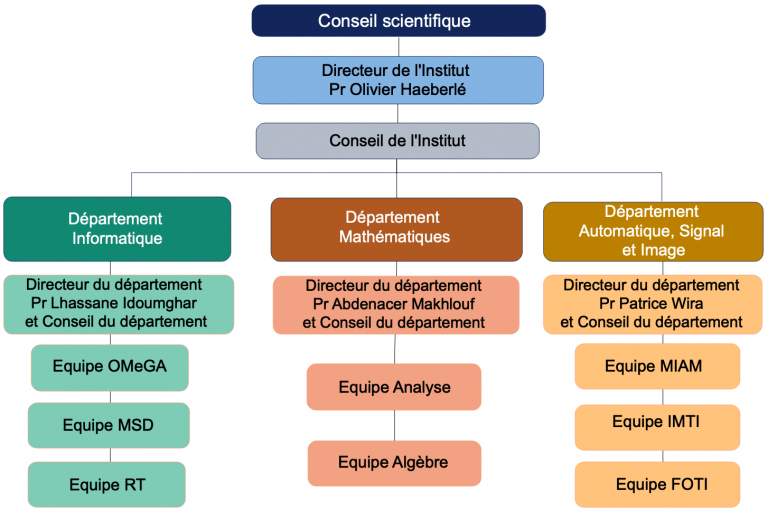
\includegraphics[width=1\textwidth]{irimas_organigramme}%
						\caption{Organigramme de l'\acrshort{IRIMAS}~\cite{IRIMAS_Organigramme}}%
						\label{fig:irimas_organigramme}%
					\end{figure}
				\paragraph*{}
					La répartition ainsi que les directeurs de ces départements sont visibles sur la figure \ref{fig:irimas_organigramme}. Durant le stage j'ai rejoint l'équipe \gls{OMeGA} du département informatique.
			\subsection{Équipe \acrshort{OMeGA}}
				\paragraph*{}
					Au sein du département informatique, l'équipe \gls{RTe} est situé à Colmar tandis que les équipe \gls{OMeGA} et \gls{MSD} sont actuellement hébergées dans l'aile sud du bâtiment Lumière de l'\gls{ENSISA} sur le campus Illberg à Mulhouse (point I sur le plan de l'annexe \ref{sec:uha_illberg_map}).
				\paragraph*{}
					L'équipe est sous la responsabilité de Lhassane Idoumghar (qui dirige aussi le département informatique) et est composée d'une douzaine de chercheurs et enseignants-chercheurs et de 5 doctorants qui travaillent essentiellement sur les axes de recherche ``Optimisation par Métaheuristiques'' et ``Algorithmique et Modélisations''.
				\paragraph*{}
					Une métaheuristique est un ensemble de concepts pouvant être utilisés pour définir des méthodes heuristiques pouvant être appliquées à un large éventail de problèmes différents, souvent des problèmes d’optimisation difficile. En d'autres termes, une métaheuristique peut être considérée comme un cadre algorithmique général qui peut être appliqué à différents problèmes d'optimisation avec relativement peu de modifications pour les adapter à un problème spécifique.
				\paragraph*{}
					``Le premier groupe de travail s’intéresse à l’algorithmique pour l’intelligence artificielle en développant de nouveaux algorithmes hybrides (basés sur des métaheuristiques à base d’agents intégrant des méthodes d’apprentissage) pour résoudre des problèmes d'optimisation mono-objectif ou multi-objectif de natures continues, discrètes et combinatoires, avec la prise en compte de l’aspect dynamique dans certains cas. L’adaptation et l’implémentation de ces futurs algorithmes hybrides sur des clusters hétérogènes de machines GPU sont également étudiées.''~\cite{IRIMAS_OMeGA}
				\paragraph*{}
					``L’activité du second groupe s’inscrit dans le thème d’analyse de données visuelles et géométriques (images, vidéo, nuages de points, courbes, etc.). Dans le cadre de cette thématique, ils développent des algorithmes et des concepts pour résoudre des problèmes de nature géométrique qui apparaissent dans de nombreuses disciplines de l’informatique [\ldots] ainsi que des techniques d’extraction d’information dans des données visuelles pour répondre à des problématiques de visualisation et d’analyses de scènes.''~\cite{IRIMAS_OMeGA}
				\paragraph*{}
					Laurent Moalic, qui a proposé le sujet de ce stage (détaillé dans la partie \ref{sec:presentation_stage}), est membre de l'équipe \gls{OMeGA}, le sujet proposé, ainsi que ces travaux en général, s’inscrivent dans l'axe Optimisation par Métaheuristiques du laboratoire.
	\chapter{Présentation du stage}\label{sec:presentation_stage}
		\section{Contexte du stage}
			\subsection{\acrshort{HEAD}}
				\paragraph*{}
					En \citeyear{Moalic2018} a été publié l'article \citetitle{Moalic2018}~\cite{Moalic2018} par \citeauthor{Moalic2018}, cet article propose l'utilisation de méthodes d'optimisation métaheuristiques hybrides sur le \gls{GVCP}.
				\paragraph*{}
					La coloration des sommets d'un graphe implique l'attribution d'une couleur à chaque sommet, de sorte que deux sommets adjacents (reliés par une arête) aient des couleurs différentes. Le \gls{GVCP} consiste à trouver le nombre minimal de couleurs, appelé nombre chromatique, requis pour colorer le graphe tout en respectant ces contraintes. La figure~\ref{fig:Petersen_graph_3-coloring} montre un exemple de solution a ce problème pour un graphe simple.
					\begin{figure}[H]
						\centering%
						
\includegraphics[width=0.25\textwidth]{Petersen_graph_3-coloring}%
						\caption{Une solution optimale au \acrshort{GVCP} pour le graphe de Petersen en utilisant 3 couleurs~\cite{wiki:Graphe_de_Petersen}}%
						\label{fig:Petersen_graph_3-coloring}%
					\end{figure}
				\paragraph*{}
					L'hybridation utilisée dans l'article pour résoudre ce problème est de type mémétique, c'est-à-dire qu'elle résulte de l'hybridation entre un algorithme génétique et un algorithme de recherche locale.
				\paragraph*{}
					Les algorithmes génétiques sont des métaheuristiques inspirées du processus de sélection naturelle qui appartiennent à la classe plus large des algorithmes évolutifs. Les algorithmes génétiques sont couramment utilisés pour générer des solutions de haute qualité aux problèmes d'optimisation et de recherche en s'appuyant sur des opérateurs inspirés de la biologie telles que la mutation, le croisement et la sélection.
				\paragraph*{}
					Les recherches locales prennent une solution potentielle à un problème et regardent ses voisins (c'est-à-dire des solutions similaires à l'exception de détails mineurs) dans l'espoir de trouver une solution améliorée. Les méthodes de recherche locales ont tendance à rester bloquées dans des régions sous-optimales ou sur des plateaux où de nombreuses solutions s’apparentent.
				\paragraph*{}
					L'algorithme proposé, \gls{HEAD}, est basé sur \gls{HEA}~\cite{Galinier1999} et fonctionne avec une population de deux individus. De plus il intègre une nouvelle façon de gérer la diversité a la population avec des solutions ``élites''. L'hybridation est faite avec une \gls{RT} adapté au \gls{GVCP}.
				\paragraph*{}
					Les \gls{RT} sont des métaheuristiques utilisant des méthodes de recherche locales en assouplissant leur règle de base. À chaque étape, des mouvements de détérioration peuvent être acceptés si aucun mouvement d'amélioration n'est disponible (comme lorsque la recherche est bloquée dans un minimum local). De plus, des interdictions (désignées par le terme tabou) sont introduites pour décourager la recherche de revenir à des solutions précédemment consultées.
				\paragraph*{}
					Les expériences menées sur un ensemble d'instance \gls{GVCP} difficiles du \gls{DIMACS}, montrent que \gls{HEAD} produit de bon résultats. Les résultats obtenus par \gls{HEAD} laissent penser que ce type d'approche pourrait être appliqué avec succès à d'autres problèmes \acrshort{NP}-complets.
				\paragraph*{}
					Les problèmes \acrshort{NP}-complets représentent les problèmes les plus difficiles de \acrfull{NP} qui est une classe de complexité utilisée pour classifier les problèmes de décision. \acrshort{NP} est l'ensemble des problèmes de décision pour lesquels chaque entrée du problème doit être associée à un ensemble de solutions de longueur polynomiale, dont la validité peut être testée rapidement (en temps polynomial).
				\paragraph*{}
					Si un problème \acrshort{NP}-complet a un algorithme en temps polynomial, tous les problèmes de \acrshort{NP} en ont. Bien qu'une solution à un problème \acrshort{NP}-complet puisse être vérifiée en temps polynomial, il n'existe aucun moyen connu de trouver une solution en temps polynomial. C'est-à-dire que le temps requis pour résoudre le problème en utilisant n'importe quel algorithme connu augmente exponentiellement avec la taille du problème. Les problèmes \acrshort{NP}-complets donc sont souvent traités en utilisant des méthodes heuristiques et des algorithmes d'approximation.
			\subsection{\acrshort{SCP} et \acrshort{USCP}}
				\paragraph*{}
					Le \gls{SCP}, fait partit des 21 problèmes \acrshort{NP}-complets de \citeauthor{Karp1972}~\cite{Karp1972}, il peut être énoncé comme suit:
				\paragraph*{}
					Étant donné un ensemble univers \(U = \{u_1, u_2, u_3, \dots, u_m\}\) et une famille \(S = \{s_1, s_2, \dots, s_n\}\) de sous-ensembles de \(U\) avec \(c_i\), coût du sous-ensemble \(s_i\), le problème consiste à trouver une sous-famille de \(S\) permettant de couvrir chaque élément de \(U\) au moins une fois avec un coût minimum. Un élément \(e\) de \(U\) est couvert par un sous-ensemble \(A\) si \(e \in A\).
				\paragraph*{}
					Dans le cas où tous les sous-ensembles \(s_i\) ont un coût identique, le problème est alors appelé \gls{USCP} ou \gls{UwSCP}, un exemple graphique d'instance d'\gls{USCP} est visible sur la figure \ref{fig:uscp_example}.
				\begin{figure}[H]
					\centering%
					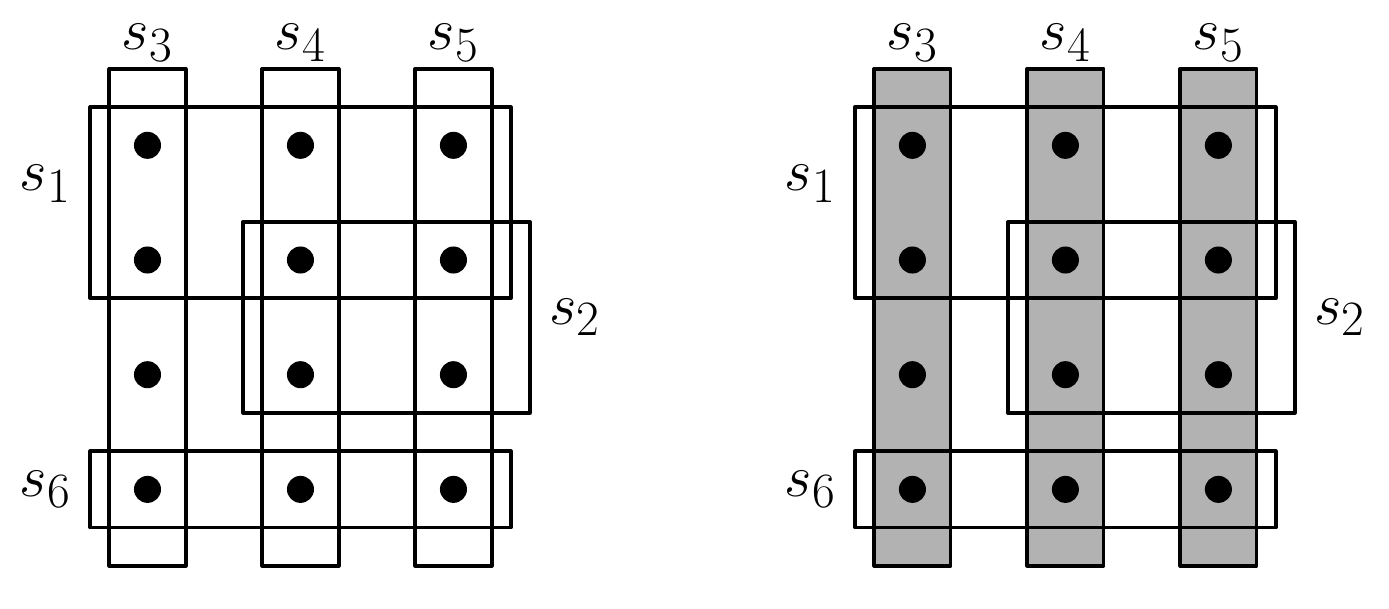
\includegraphics[width=0.65\linewidth]{uscp_example}%
					\caption{Exemple d'instance du \acrshort{USCP} et solution optimale (ensembles grisés)~\cite{Mount2017}}%
					\label{fig:uscp_example}%
				\end{figure}
				\paragraph*{}
					En général les instances de \gls{SCP} sont définies par une matrice d'incidence \(A = \left(a_{i,j}\right)\) de taille \(m \times n\) avec
					\[\forall i \in \{1,\ldots,m\},\ \forall j \in \{1,\ldots,n\},\ a_{i,j} = \left\{
						\begin{array}{ll}
							1 & \text{si } u_i \in s_j \\
							0 & \text{sinon}
						\end{array}
					\right.\]
					\(a_{i,j} = 1\) signifiant donc que le point \(u_i\) est couvert par le sous-ensemble \(s_j\), ainsi qu'un vecteur coût \(n\)-dimensionnel \(c = \left(c_j\right)\) avec \(\forall j \in N\), \(c_j\) le coût du sous-ensemble \(j\).
				\paragraph*{}
					Les solutions sont quant à elles définies par un vecteur \(n\)-dimensionnel \(x = \left(x_j\right)\) avec
					\[\forall j \in \{1,\ldots,n\},\ x_j = \left\{
						\begin{array}{ll}
							1 & \text{si } u_i \text{ fait parti de la solution}\\
							0 & \text{sinon}
						\end{array}
					\right.\]
					le coût de la solution étant égal à
					\[\sum_{j \in \{1,\ldots,n\}}{c_j x_j}\]
					et la solution étant valide si
					\[\forall i \in \{1,\ldots,m\}\ ,\sum_{j \in \{1,\ldots,n\}}{a_{ij}x_j} \ge 1\]
				\paragraph*{}
					Par exemple, l'instance suivante, définie par la matrice d'incidence \(A\) et le vecteur coût \(c\) a comme solution optimale le vecteur \(x\):
					\[
					\begin{blockarray}{ccccccccc}
						& s_1 & s_2 & s_3 & s_4 & s_5 & s_6 & s_7\\
						\begin{block}{c(ccccccc)c}
							    & 0 & 1 & 1 & 0 & 0 & 0 & 1 & u_1\\
							    & 0 & 0 & 1 & 0 & 1 & 1 & 0 & u_2\\
							A = & 1 & 1 & 0 & 1 & 0 & 1 & 0 & u_3\\
							    & 0 & 0 & 0 & 0 & 1 & 1 & 1 & u_3\\
							    & 1 & 0 & 1 & 0 & 0 & 0 & 1 & u_4\\
						\end{block}
						\\
						\begin{block}{c(ccccccc)c}
							c = & 3 & 1 & 2 & 4 & 1 & 2 & 1 &\\
						\end{block}
						\\
						\begin{block}{c(ccccccc)c}
							x = & 0 & 1 & 1 & 0 & 0 & 0 & 1 &\\
						\end{block}
					\end{blockarray}
					\]
				\paragraph*{}
					Il est à noté que, bien que le \gls{USCP} soit un cas particulier du \gls{SCP}, du fait de l'information réduite de par l’absence de poids pour les sous-ensembles, il est généralement considéré que le \gls{USCP} est plus difficile à résoudre que le \gls{SCP}~\cite{Yelbay2015}.
		\section{Objectifs du stage}
			\subsection{Objectif initial}
				\paragraph*{}
					L'objectif du stage est de développer des algorithmes hybrides avec une recherche poussée de performance pour le \gls{USCP}, la piste première à explorer étant d'utiliser les principes de \gls{HEAD} et de les adapter au \gls{USCP}.
				\paragraph*{}
					Le développement d'algorithmes méthaheuristique se faisant en se basant sur les travaux existant, il sera nécessaire d'analyser la littérature du problème afin d'identifier les recherches locales, opérateur de sélection, opérateurs de croisement et mutation efficaces pour le problème afin de les comparer et de sélectionner les plus adaptés pour notre algorithme.
				\paragraph*{}
					Pour réaliser ces comparaison et afin d'évaluer la performance de notre algorithme, il sera nécessaire d'identifier les instances de benchmark classiques de la littérature ainsi que les résultats obtenus par les méthodes les plus efficaces connues afin de ce comparer à ces dernières.
				\paragraph*{}
					Une fois toutes ces recherches réalisées, le développement pourra commencer, dans un premier temps il faudra implémenter les structures et algorithmes de base lié au \gls{SCP}, puis il faudra implémenter la recherche locale que nous utiliserons dans notre hybridation et enfin implémenter l'algorithme en lui même.
				\paragraph*{}
					Après cela viendra la phase de réglage ou il faudra alterner entre benchmarks, optimisation logicielle et variation des paramètres et composants de l'algorithme afin optimiser son efficacité. Une fois les réglages terminé, une étude comparative de la performance de l'algorithme sera réalisé.
			\subsection{Objectifs supplémentaires}
				\paragraph*{}
					Après que la première version notre algorithme ai été conçut et implémenté (voir section \ref{sec:memetic_algorithm} pour le détail des différentes versions de l'algorithme), nous avons commencé à obtenir de bon résultats, il a donc été décidé de soumettre à la conférence \acrshort{ROADEF2020} qui est le ``\acrlong{ROADEF2020}''.
				\paragraph*{}
					La deuxième version de l'algorithme a été développé et a servit pour la publication pour \acrshort{ROADEF2020}, les résultats de cette nouvelle version étant encore meilleurs et apportant une contribution assez significative, il a été décidé de soumettre à la conférence \acrshort{LION14} qui est la ``\acrlong{LION14}''.
				\paragraph*{}
					Enfin, le dernier objectif qui fut ajouté est d'utiliser l'algorithme développé au cour du stage afin de résoudre des instances de \gls{GVCP} à partir de solutions sous-optimales qui sont générées de façon très rapide par l'algorithme de Laurent.
				\paragraph*{}
					Ces nouveaux objectif ayant été ajouté durant le stage, ils nécessitent de déjà connaitre ce qui à été réalisé durant le stage avant leur ajout, ils seront donc explicité plus en détail avec le travail réalisé durant le stage dans la section \ref{sec:work}.
		\section{Organisation du stage}
			\subsection{Environnement de travail}
				\paragraph*{}
					Un bureau avec poste informatique, proche des autres membres de l'équipe, m'a été attribué, il est partagé avec Dominique Schmitt, enseignant-chercheur sur l'axe Algorithmique et Modélisations de l'équipe \gls{OMeGA}. Dans la même zone du bâtiment se trouve les bureaux de Laurent Moalic, Mathieu Brévilliers et Julien Lepagnot avec qui j'ai le plus travaillé sur la partie recherche du stage.
				\paragraph*{}
					La nature du stage le permettant (pas de problèmes de confidentialité), j'ai décider de travailler sur mon ordinateur personnel, ce dernier est assez bien équipé pour développer et tester en local le \solver{} (programme ou sera implémenter les différents algorithmes de résolution). Il est équipé d'un Intel Core i7-4710MQ (Quad-Core 2.5 GHz / 3.5 GHz Turbo - cache 6 Mo) avec 16 Go de mémoire vive DDR3L. Le \solver{} développé n'utilise pas le GPU et ne nécessite que peut d'espace disque.
				\paragraph*{}
					Les programmes ont majoritairement été développé sur Linux, plus précisément la distribution Debian unstable (connu aussi sous le nom de code Sid), qui est très adapté au développement logiciel car renfermant les paquets les plus récents qui viennent d'être introduits dans le système Debian (voir annexe \ref{sec:programs_versions} pour les versions des différents programmes utilisés).
				\paragraph*{}
					Le programmes ont été développés en \Cpp{}17\footnote{Révision de 2017 du \href{https://www.iso.org/standard/68564.html}{standard ISO/IEC 14882}}, conçu pour fonctionner sur Linux et Windows et pour embarquer toutes leur dépendances afin d’être autonome. Ils utilisent \textit{CMake} comme build-system et \textit{Make} ou \textit{Ninja} comme sous-système et sont compilables en utilisant \textit{gcc} et \textit{clang} sous Linux et \textit{Microsoft Visual \Cpp{} compiler} sous Windows. Le support de plusieurs plateformes d'exécution et compilateurs n'était pas nécessaire pour ce projet mais facilement atteignable, j'ai donc décidé de le prendre en compte pour que mon travail soit le plus facile possible à utiliser et reprendre.
				\paragraph*{}
					Le développement c'est fait sur Linux en utilisant l'\gls{IDE} \textit{CLion} tandis que la vérification de la compilation et compatibilité Windows c'est fait avec l'\gls{IDE} \textit{Microsoft Visual Studio}. La rédaction des différent scripts de lancement des benchmarks ont été rédigés avec l'éditeur \textit{Sublime Text}.
				\paragraph*{}
					Le code du projet est formaté en utilisant \textit{clang-format} avec un style personnalisé et est fréquemment analysé avec l'analyseur statique \textit{clang-tidy} afin d'éviter au maximum les erreurs de code du à une inattention ou une faute de frappe.
				\paragraph*{}
					Le code, les données et les documents du projet ont été versionné avec \textit{git} dans 4 dépôts:
					\begin{description}
						\item[USCP] contient le code et les ressources des différent programmes développés
						\item[USCP\_instances] contient les instances de benchmark utilisées ainsi que de la documentation sur ces dernières
						\item[USCP\_results] contient les résultats des différent benchmarks réalisés ainsi que de la documentation sur ces derniers
						\item[UTBM\_ST50\_Rapport\_de\_stage\_IRIMAS] contient les rapport et présentations demandées par l'\gls{UTBM} et l'\gls{UQAC}, notamment les rapports de stage
					\end{description}
					Chacun de ses dépôt a pour \textit{remote} un dépôt GitHub privé afin de toujours avoir une sauvegarde en cas d'accident.
			\subsection{Cluster \acrshort{HPC}}
				\paragraph*{}
					Le méso-centre de l'Université de Strasbourg se situe parmi les 4 centres de calcul régionaux les plus puissants en France. Il est opéré par le pôle \gls{HPC} de la Direction du numérique de l’Université de Strasbourg~\cite{UNISTRA_Calcul_scientifique}. Au cour de la 6ème semaine du stage j'ai obtenu l’accès à la partition ``public'' au cluster \gls{HPC} du service de calcul scientifique du méso-centre de Strasbourg.
				\paragraph*{}
					Les ressources de calcul du \gls{HPC} auquel j'ai eu accès sont composées de 1.3Po (1\,266\,700Go) de stockage, 9\,968 cœurs de calcul, environ 47To (47\,818Go) de mémoire vive, le tout réparti sur 467 nœuds de calcul. Parmi les nœuds, on compte notamment:
					\begin{itemize}
						\item 56 noeuds Intel Xeon Nehalem/Westmere à 24Go de RAM, financés par mutualisation
						\item 145 noeuds Intel Xeon Sandy-Bridge à 16 coeurs et 64Go de RAM, financés par l'\gls{Equip@meso} avec le soutien du conseil scientifique de l'Université de Strasbourg
						\item 150 noeuds Intel Sandy et Ivy Bridge, Westmere de 16 ou 24 cœurs et de 64 à 128Go de RAM, financés par mutualisation
					\end{itemize}
					Tous les processeurs sont d'architecture x86\_64, et les nœuds de login et de calculs utilisent \textit{Scientific Linux} 7.5\footnote{Équivalent RedHat même version, voir \url{http://www.scientificlinux.org/}}.
				\paragraph*{}
					Le cluster \gls{HPC} a servit à réaliser l'ensemble des benchmarks du projet, ces benchmarks demandant énormément d'heures de calcul (voir sec \ref{sec:analyse_stage_travail}), il n'aurais pas été possible d'avoir des données aussi conséquentes sur lesquelles travailler sans cet accès au méso-centre.
				\paragraph*{}
					Après que l'équipe en charge du méso-centre ai installé notre clé ssh sur le noeud de login, l'accès au cluster \gls{HPC} se fait en ssh. L'utilisation des noeuds de calcul se fait par l'intermédiaire de \textit{Slurm Workload Manager} qui gère les différent noeuds, partitions de calcul, groupes d'utilisateurs, \ldots{} et gère la répartitions des taches (appelées job) par un système de priorités et de files d'attentes.
				\paragraph*{}
					Différents programmes sont mis a disposition sur le cluster par l'intermédiaire de \textit{GNU Modules} qui permet de les charger. Les deux modules utilisé durant le stage sont \texttt{cmake/cmake-3.12.2} et \texttt{gcc/gcc-9} pour la compilation des programmes.
				\paragraph*{}
					Le code des programmes développés est récupéré sur le cluster avec \textit{git} par l'intermédiaire des dépôts privés sur Github tandis que les résultats de l’exécution du \solver{} pour les différents benchmarks sont téléchargés du cluster avec \textit{rsync}.
	\printbibliography[heading=bibintoc]{}
	\printglossary[type=\acronymtype,nogroupskip=true,title=Lexique,toctitle=Lexique]{}
	\chapter*{Annexes}\addcontentsline{toc}{chapter}{Annexes}\markboth{Annexes}{}
		\setcounter{section}{0}
		\renewcommand{\thesection}{\Alph{section}}
		\renewcommand{\theHsection}{appendixsection.\Alph{section}}
		\section{Centres de formations de l'\acrshort{UHA}}\label{sec:uha_formation}
			\paragraph*{}
				%!TEX encoding = UTF-8 Unicode

\begin{tabularx}{\linewidth}{lX}
	\toprule
	\multicolumn{2}{c}{Unités de Formation et de Recherche}\\
	\midrule
	\acrshort{FLSH} & \acrlong{FLSH} de Mulhouse\\
	\acrshort{FSESJ} & \acrlong{FSESJ} de Mulhouse\\
	\acrshort{FST} & \acrlong{FST} de Mulhouse\\
	\acrshort{FMA} & \acrlong{FMA} de Colmar\\
	\bottomrule
\end{tabularx}

				\hfill\\
			\paragraph*{}
				%!TEX encoding = UTF-8 Unicode

\begin{tabularx}{\linewidth}{lX}
	\toprule
	\multicolumn{2}{c}{Instituts et Écoles d’ingénieur}\\
	\midrule
	\acrshort{ENSCMu} & \acrlong{ENSCMu} de Mulhouse\\
	\acrshort{ENSISA} & \acrlong{ENSISA} de Mulhouse\\
	\acrshort{IUT} de Mulhouse & \acrlong{IUT} de Mulhouse\\
	\acrshort{IUT} de Colmar & \acrlong{IUT} de Colmar\\
	\bottomrule
\end{tabularx}

				\hfill\\
			\paragraph*{}
				%!TEX encoding = UTF-8 Unicode

\begin{tabularx}{\linewidth}{lX}
	\toprule
	\multicolumn{2}{c}{Services de formation et certifications}\\
	\midrule
	\acrshort{CFAU} & \acrlong{CFAU}\\
	\acrshort{CUFEF} & \acrlong{CUFEF}\\
	\acrshort{SERFA} & \acrlong{SERFA}\\
	\acrshort{CLAM} & \acrlong{CLAM}\\
	\bottomrule
\end{tabularx}

				\hfill\\
		\newpage\section{Laboratoires de l'\acrshort{UHA}}\label{sec:uha_laboratories}
			\paragraph*{}
				%!TEX encoding = UTF-8 Unicode

\begin{tabularx}{\linewidth}{lX}
	\toprule
	\multicolumn{2}{c}{Pôle Chimie, Physique, Matériaux et Environnement}\\
	\midrule
	\acrshort{GRE} & \acrlong{GRE}\\
	\acrshort{IPHC} & \acrlong{IPHC}\\
	\acrshort{S2M} & \acrlong{S2M}\\
	\acrshort{LIMA} & \acrlong{LIMA}\\
	\acrshort{LPIM} & \acrlong{LPIM}\\
	\acrshort{LVBE} & \acrlong{LVBE}\\
	\bottomrule
\end{tabularx}

				\hfill\\
			\paragraph*{}
				%!TEX encoding = UTF-8 Unicode

\begin{tabularx}{\linewidth}{lX}
	\toprule
	\multicolumn{2}{c}{Pôle Sciences pour l'Ingénieur}\\
	\midrule
	\acrshort{IRIMAS} & \acrlong{IRIMAS}\\
	\acrshort{LPMT} & \acrlong{LPMT}\\
	\bottomrule
\end{tabularx}

				\hfill\\
			\paragraph*{}
				%!TEX encoding = UTF-8 Unicode

\begin{tabularx}{\linewidth}{lX}
	\toprule
	\multicolumn{2}{c}{Pôle Sciences Humaines et Sociales}\\
	\midrule
	\acrshort{ARCHIMEDE} & \acrlong{ARCHIMEDE}\\
	\acrshort{BETA} & \acrlong{BETA}\\
	\acrshort{CERDACC} & \acrlong{CERDACC}\\
	\acrshort{CREGO} & \acrlong{CREGO}\\
	\acrshort{CRESAT} & \acrlong{CRESAT}\\
	\acrshort{ILLE} & \acrlong{ILLE}\\
	\acrshort{LISEC} & \acrlong{LISEC}\\
	\acrshort{SAGE} & \acrlong{SAGE}\\
	\bottomrule
\end{tabularx}

				\hfill\\
		\newpage\section{Plan du campus Illberg de l'\acrshort{UHA}}\label{sec:uha_illberg_map}
			\begin{figure}[H]
				\centering%
				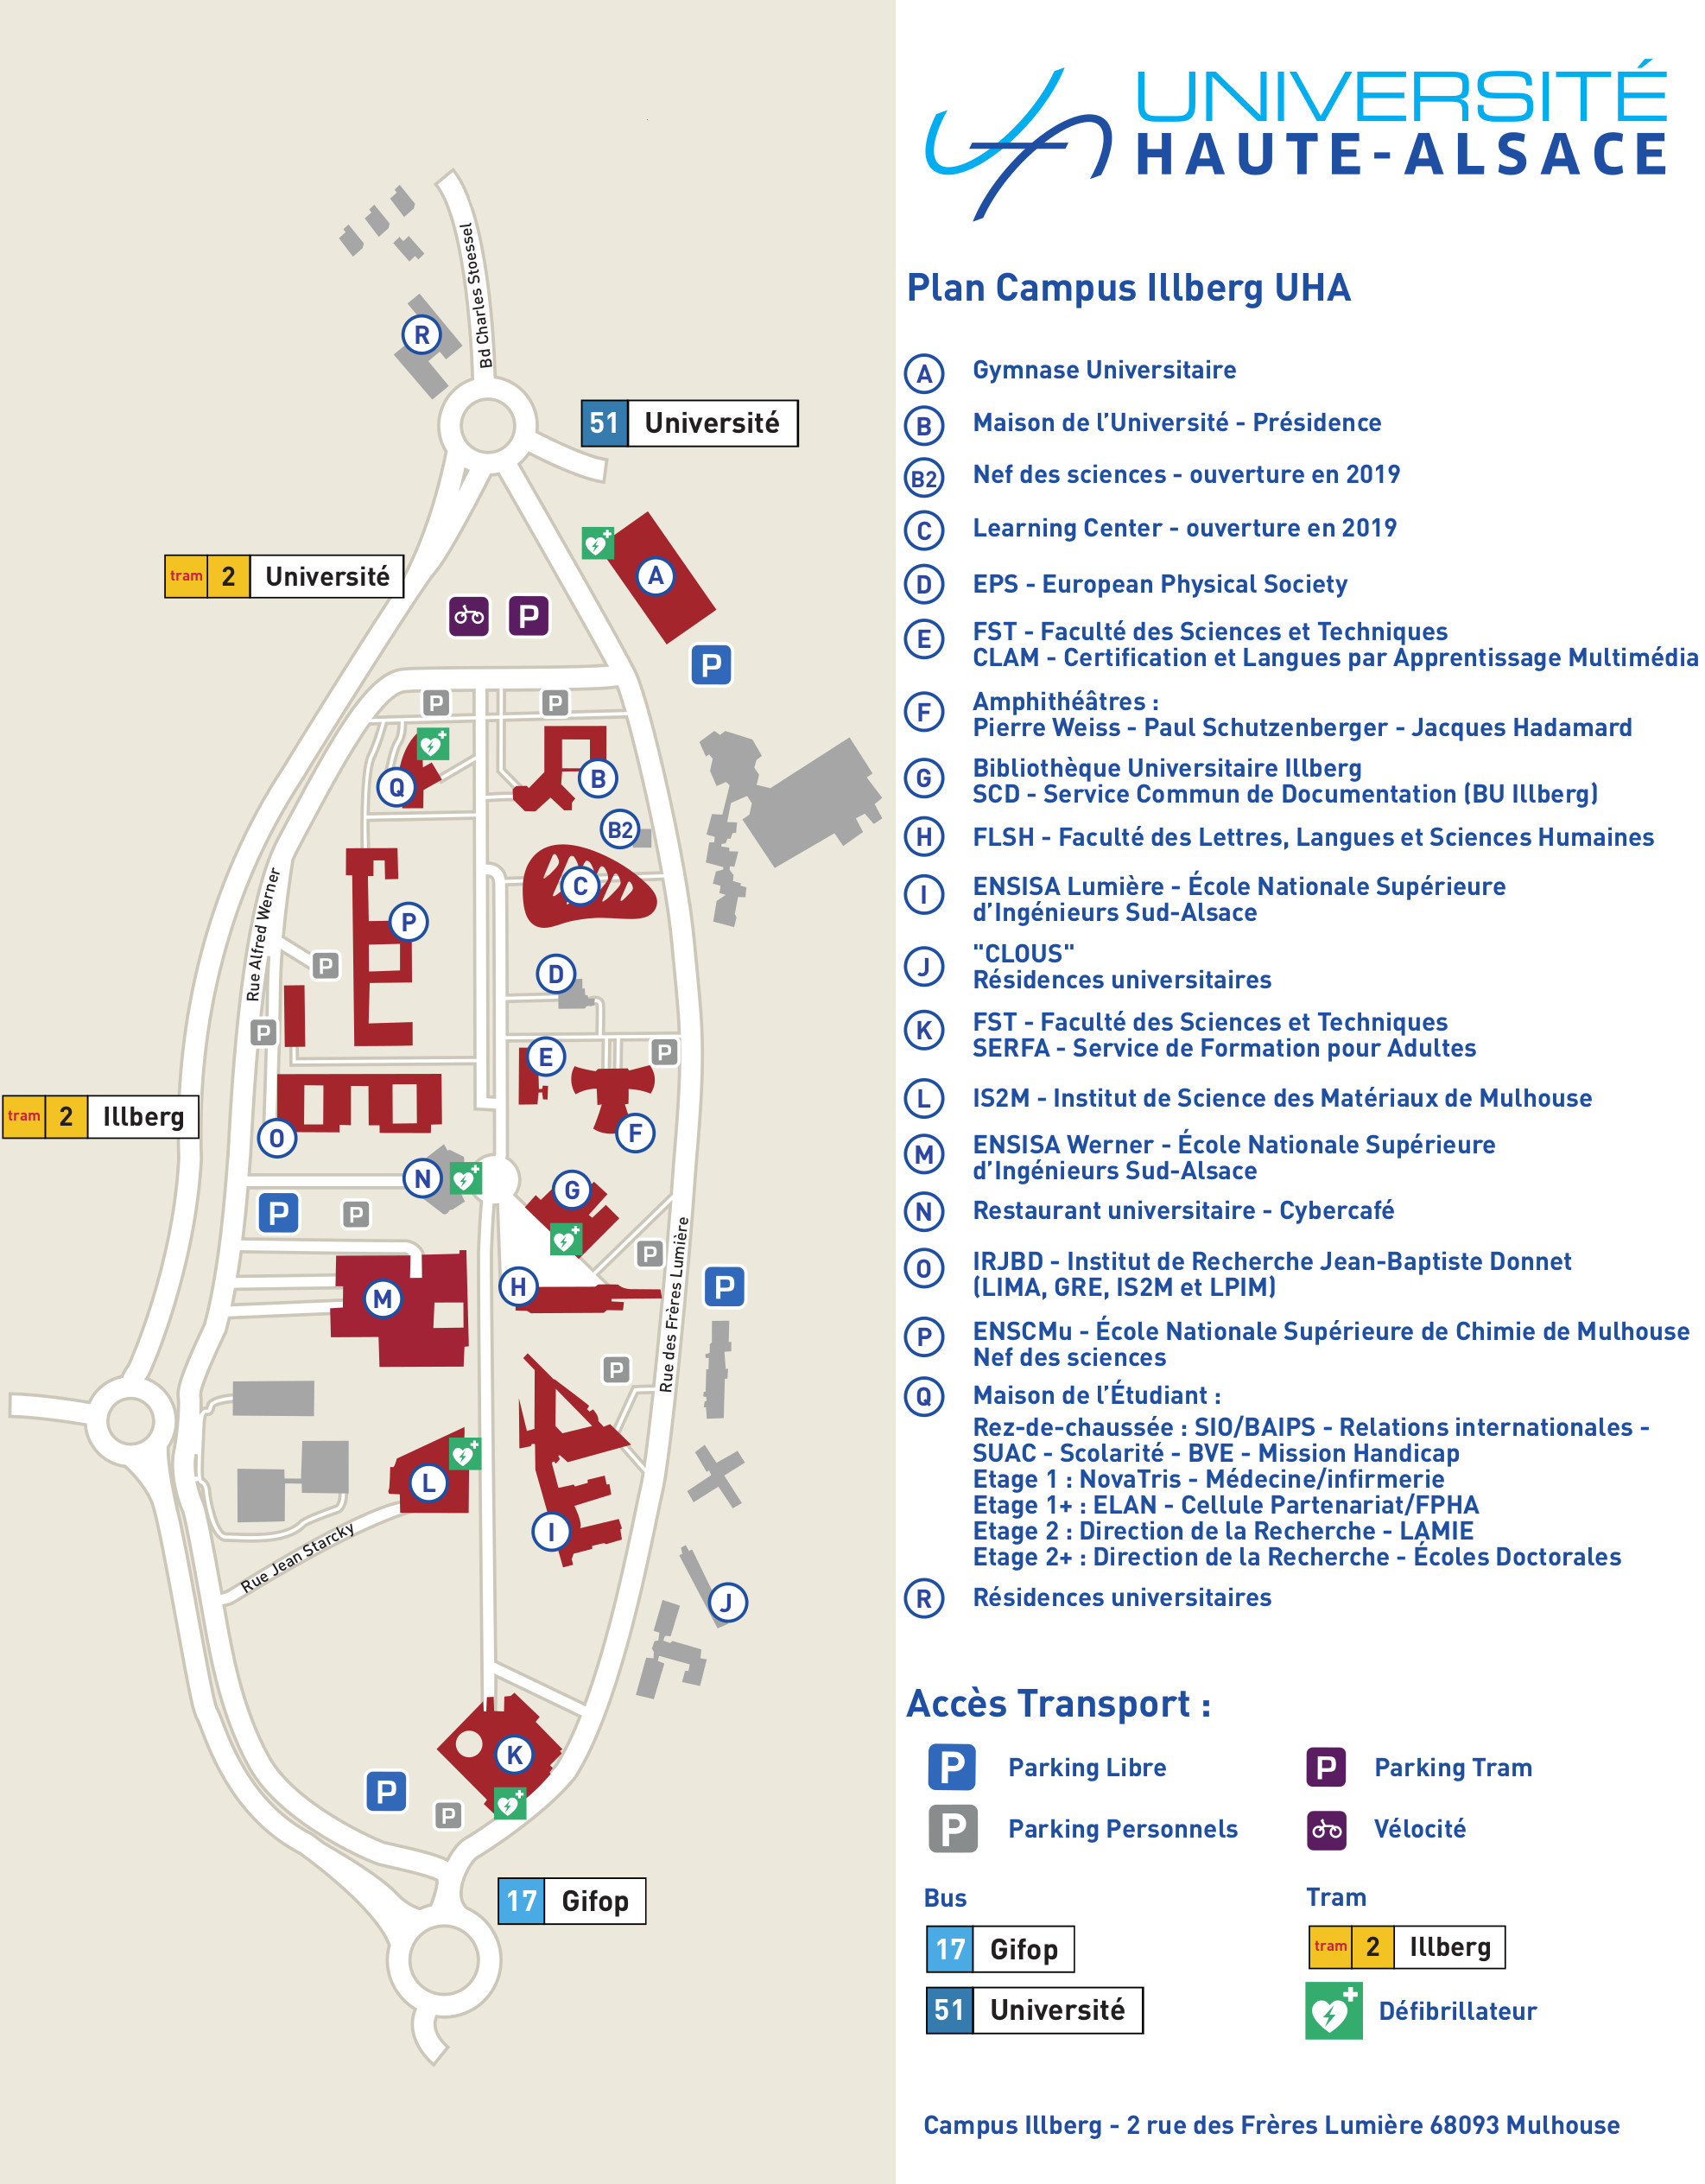
\includegraphics[width=0.95\textwidth]{UHA_plan_campus_Illberg}%
				\caption{Plan du campus Illberg de l'\acrshort{UHA}~\cite{UHA_Plan_acces}}%
				\label{fig:UHA_plan_campus_Illberg}%
			\end{figure}
		\newpage\section{Versions des programmes utilisés}\label{sec:programs_versions}
			\paragraph*{Sur plusieurs machines/environnements}
				\begin{center}
					\begin{tabular}{lccc}
						& HPC (Linux) & Local (Linux) & Local (Windows)\\
						\midrule
						git & 1.8.3.1 & 2.25.0 & TODO\\
						CMake & 3.12.2 & 3.15.4 & TODO\\
						Make & 3.82 & 4.2.1 & TODO\\
						Ninja & --- & 1.9.0 & TODO\\
						gcc & 9.2 & 9.2.1 & TODO\\
						clang & --- & 8.0.1 & TODO\\
						rsync & 3.0.9 & 3.1.3 & ---\\
					\end{tabular}
				\end{center}
			\paragraph*{Sur la machine locale (Linux)}
				\begin{itemize}
					\item CLion 2019.3.2
					\item Sublime Text Build 3211
					\item clang-format 8.0.1
					\item clang-tidy 8.0.1
				\end{itemize}
			\paragraph*{Sur la machine locale (Windows)}
				\begin{itemize}
					\item MSVC TODO
				\end{itemize}
			\paragraph*{Sur le cluster \gls{HPC} du méso-centre de Strasbourg}
				\begin{itemize}
					\item Slurm 15.08.13
					\item Modules 3.2.10
				\end{itemize}
	\makeutbmbackcover{}
\end{document}
